\section{Implementation}\label{sec:implementaion}
%To demonstrate the use of Crypt$\epsilon$ primitives let us look at the following example.
\label{implementation}
In this section we describe the implementation of Crypt$\epsilon$. First we discuss our novel proposed technique for extending the $labMult$ operation of \textsf{labHE} to support $n > 0$ multiplicands. Then we describe the implementations for each primitive. Last, we use the example programs from the previous section to illustrate the performance of \system.

\subsection{\textbf{General n-way Multiplication for \textsf{labHE}}}\label{genlab}
In addition to the operations supported by a \textsf{LHE}  scheme, \textsf{labHE} supports multiplication of two labeled ciphers. 
\\ $\bullet \textbf{labMult}(\mathbf{c}_1,\mathbf{c}_2)$ -
On input two labeled ciphers $\mathbf{c}_1=(a_1,d_1)$ and $\mathbf{c}_2=(a_2,d_2)$, it computes a "multiplication" ciphertext $\mathbf{e}=labMult(\mathbf{c_1,c_2})=Enc_{pk}(a_1,a_2)\oplus cMult(d_1,a_2) \oplus cMult(d_2,a_1)$. Observe that $Dec_{sk}(\mathbf{e})=m_1\cdot m_2 -b_1 \cdot b_2$.\\
 $\bullet \textbf{labMultDec}_{sk}(d_1,d_2,\mathbf{e})$ - On input two encrypted masks $d_1,d_2$ of two labHE ciphers $\mathbf{c_1},\mathbf{c_2}$ and the output $\mathbf{e}$ of $labMult(\mathbf{c_1},\mathbf{c_2})$, it decrypts the product as $m_3=Dec_{sk}(\mathbf{e})+Dec_{sk}(d_1)\cdot Dec_{sk}(d_2) = m_1\cdot m_2$ .   \\
In this paper we propose an efficient way of extending the $labMult$ operation for a $n$-way multiplication.
\begin{algorithm}
\caption{$genLabMult$ - generate label for $labMult$}
\begin{algorithmic}[1]
\STATEx
\textbf{Input}: $\mathbf{c_1}=labEnc_{pk}(m_1)=(a_1,d_1)$  where\STATEx $\hspace{0.9cm} a_1= m_1-b_1, d_1=Enc_{pk}(b_1)$\STATEx $\hspace{0.9cm} \mathbf{c_2}=labEnc_{pk}(m_2)$
\STATEx$\hspace{0.9cm} a_2= m_2-b_2, d_2=Enc_{pk}(b_2)$
\STATEx \textbf{Output}: $\mathbf{e}=labEnc_{pk}(m_1\cdot m_2)$ 
\STATEx \textbf{\textsf{AS}:} \STATE Computes $\textbf{e}'=labMult(\mathbf{c_1,c_2}) \oplus Enc_{pk}(r)$ where $r$ is a random mask \STATE Sends $\mathbf{e'},\mathbf{c_1},\mathbf{c_2}$ to \textsf{CSP}
\STATEx \textbf{\textsf{CSP}:}
\STATE Decrypts $\mathbf{e'}$, to get $Dec_{sk}(\mathbf{e}')=m_1\cdot m_2 -b_2\cdot b_1 + r$
\STATE Computes $b_1 \cdot b_2$ from $d_1$ and $d_2$.
\STATE Removes $b_1\cdot b_2$ from $e'$ to compute $e''=m_1\cdot m_2+r$
\STATE Picks a seed $\sigma'$ and label $\tau'$
\STATE Computes $\bar{a}=e''-b'=m_1\cdot m_2 +r -b'$, $b'=\mathcal{F}(\sigma',\tau')$ and $d'=Enc_{pk}(b')$
\STATE Send $\bar{e}=(\bar{a},d')$ to \textsf{AS}\STATEx \textbf{\textsf{AS}:}
\STATE Computes true cipher $\mathbf{e}=(a',d')$ where $a'=\bar{a}-r=m_1\cdot m_2 - b'$
 \end{algorithmic}
\end{algorithm}
Consider the case where we want to multiply the respective ciphers of  $n$ messages $\{m_1,...m_n\} \in \mathcal{M}^n$. Note that the reason why we can't simply use $labMult$ for a generic $n-$ way multiplication is because, the "multiplication" cipher $\mathbf{e}=labMult(\mathbf{c_1},\mathbf{c_2})$ does not have  a corresponding label. Thus for generalizing the $labMult$ operation for $n$ multiplicands what we have to do is to generate a label and a seed for every intermediary product of two multiplicands. This can be done as shown by Algorithm 1. Note that the mask $r$ protects the value of $m_1\cdot m_2$ from the \textsf{CSP} in step 5. Similarly since $b'$ is not known to the \textsf{AS}, $m_1\cdot m_2$ remains hidden from the \textsf{AS} in step 9. Now with the true \textsf{labHE} cipher $\mathbf{c}=(a',d')$ for the product the \textsf{AS} can compute further multiplications on it.
For a generic $n-way$ multiplication the order of multiplication can be, in fact, parallelized as  shown in Figure ~\ref{genlab-fig} to require a total of $\lceil \log n\rceil$ rounds of communication with the \textsf{CSP}.
\begin{figure}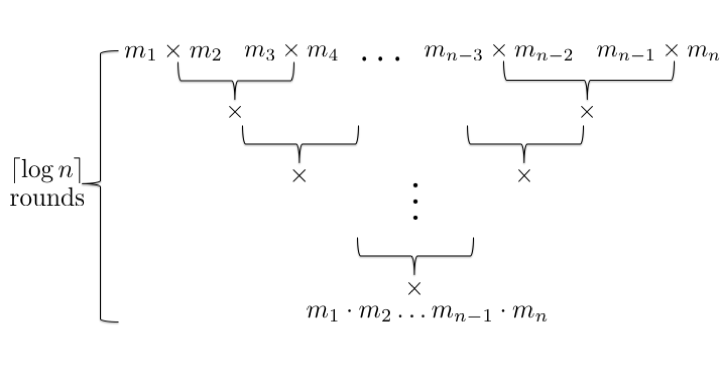
\includegraphics[height=4cm,width=8cm]{kk.png} \caption{ $genLabMult()$ - Batching of multiplicands for \textsf{labHE}} \label{genlab-fig}\end{figure}\\
\subsection{Primitive Implementation}
%Now let us explain the implementation details of the aforementioned Crypt$\epsilon$ primitives.  
In this section we explain the implementation details of two of the aforementioned \system primitives, the rest are covered in appendix section B.\\ (1)\textbf{ \textsf{GroupByCount }}$\groupbystar_A(\mathbf{\tilde{T}})$- The \textsf{GroupByCount} primitive is implemented by Algorithm ~\ref{groupby-imp}. \begin{algorithm}
\small
\caption{\textsf{GroupByCount }$\groupby_A(\mathbf{\tilde{T}})$}
\begin{algorithmic}[1]
\STATEx
\textbf{Input}: $\mathbf{\tilde{T}}$
\STATEx \textbf{Output}: $\tilde{\encV}$
\STATEx \textbf{\textsf{AS}:} \STATE Computes $\mathbf{V}=\groupbystar_{A}(\encT)$.
\STATE Masks the encrypted histogram $\mathbf{V}$ for attribute $A$ as follows \begin{gather*}\boldsymbol{\mathcal{V}}[i]= \mathbf{V}[i] \oplus labEnc_{pk}(M[i])\\M[i] \in_R [m], i \in [|V|]\end{gather*}
\STATE Sends $\boldsymbol{\mathcal{V}}$ to \textsf{CSP}.
\STATEx \textbf{\textsf{CSP}:}
\STATE Decrypts  $\boldsymbol{\mathcal{V}}$ as $\mathcal{V}[i]=labDec_{sk}(\boldsymbol{\mathcal{V}})$.\STATE Converts each entry of $\mathcal{V}$ to its corresponding one-hot-coding and encrypts it. \begin{gather*}\boldsymbol{\tilde{\mathcal{V}}}[i]=labEnc_{pk}(\tilde{\mathcal{V}[i]})\end{gather*} 
\STATE Sends $\boldsymbol{\tilde{\mathcal{V}}}$ to \textsf{AS}.
\STATEx \textbf{\textsf{AS}}:
\STATE  Rotates every entry by its corresponding mask value to obtain the desired  encrypted one-hot-coding $\boldsymbol{\tilde{V}}[i]$. \begin{gather*}\boldsymbol{\tilde{V}}[i]=RightRotate(\boldsymbol{\tilde{\mathcal{V}}},M[i])\end{gather*} 
 \end{algorithmic} \label{groupby-imp}
\end{algorithm} 
In the first step the \textsf{AS} uses the $\textsf{GroupByCount}^*$ primitive to generate the encrypted histogram $\encV$ for attribute $A$. Note that since each entry of $\mathbf{V}$ is a count of records, its value ranges from $\{0,...,m\}$. The \textsf{AS} then masks $\encV$ (step 2) and sends it to the \textsf{CSP}. The purpose of this mask is to hide the true histogram from the \textsf{CSP}. Next the \textsf{CSP} generates the encypted one-hot-coding representation for this masked histogram $\boldsymbol{\tilde{\mathcal{V}}}$ (steps 4-5) and returns it back to the \textsf{AS}. Notice that each entry of $\boldsymbol{\tilde{\mathcal{V}}}$ is a $m$-lengthed vector. The \textsf{AS} can simply rotate $\boldsymbol{\tilde{\mathcal{V}}}[i], i \in [|V|]$ by its respective mask value $M[i]$ (step 7) and get back the true encrypted histogram in one-hot-coding $\tilde{\encV}$.
Note that the \textsf{GroupByCount} primitive could have an alternative implementation using a Yao's garbled circuit that takes an input the encrypted vector and outputs the corresponding one-hot-coding representation. However this would require the circuit to decrypt and re-encrypt $O(m)$ data inside it which would be computationally heavy for larger values of $m$. 
 \\ (2)\textbf{ \textsf{Laplace }}$\lap_{\epsilon,\Delta}(\mathbf{V})$ -  
\begin{algorithm}
\small
\caption{\textsf{Laplace }$\lap_{\epsilon,\Delta}(\mathbf{V})$}
\begin{algorithmic}[1]
\STATEx
\textbf{Input}: $\encV$
\STATEx \textbf{Output}: $\hat{V}$
\STATEx \textbf{\textsf{AS}:} \STATE Generates a noisy vector $\hat{\encV}$  as \begin{gather*}\hat{\mathbf{V}}[i] = \mathbf{V}[i]\oplus labEnc_{pk}(\eta[i]),\\ \eta \sim [Lap(\frac{1}{\epsilon})]^{|V|}, i \in [|V|] \end{gather*}
\STATE Sends $\hat{\mathbb{\mathcal{V}}}$  to \textsf{CSP}
\STATEx \textbf{\textsf{CSP}:}
\STATE Decrypts $\mathbf{\hat{\mathcal{V}}}$ to get $\hat{\mathcal{V}}[i]=labDec_{sk}(\mathbf{\hat{\mathcal{V}}}[i]), i \in [|V|]$
\STATE Generates a the final noisy vector $\hat{V}$ as follows 
\begin{gather*} \hat{V}[i]=\hat{\mathcal{V}}[i]+\eta'[i], i \in [|V|], \eta' \sim [Lap(\frac{1}{\epsilon})]^{|\hat{V}|} \end{gather*}
\STATE Returns $\hat{V}$ to \textsf{AS}
 \end{algorithmic} \label{lap}
\end{algorithm} The implementation for the \textsf{Laplace} primitive is given by Algorithm ~\ref{lap}. Recall that both \textsf{AS} and \textsf{CSP} have to add Laplace noise to the output in Crypt$\epsilon$. Hence the \textsf{Laplace} primitive has two phase. In the first phase,  the \textsf{AS} adds an instance of encrypted Laplace noise to the encrypted input (step 1 in Algorithm ~\ref{lap}) to generate $\mathbf{\hat{\mathcal{V}}}$. This acts as the input to the second phase which is executed by the \textsf{CSP}. Here the \textsf{CSP} decrypts $\mathbf{\hat{\mathcal{V}}}$ and adds a second instance of the Laplace noise to generate the final noisy output $\hat{V}$ in the clear (steps 3-4). The \textsf{Laplace} primitive with an encrypted scalar $\encC$ as the input is implemented in a similar way. 

\subsection{Classification of \system Programs}
Crypt$\epsilon$ programs can be classified into three classes based on the number and type of interaction required between the \textsf{AS} and the \textsf{CSP}.  \\
(1)\stitle{ \textbf{Class I - Single Decrypt Interaction Programs:}}\\
Recall that the output of all the transformation primitives are encrypted.  Since  the \textsf{CSP} has exclusive access to the secret key, it is the only entity in the Crypt$\epsilon$ setting capable of decryption. Thus for releasing any result (albeit noisy) in the clear, we need to interact at least once with the \textsf{CSP} so that it can decrypt the encrypted noisy answer. Crypt$\epsilon$ supports this type of interactions via the two measurement primitives. Some Crypt$\epsilon$ programs require only this one round of interaction at the very end to release the noisy output. All other transformations can be performed by the \textsf{AS} via homomorphic operations on the encrypted data records. Typically these programs are counting queries on a single attribute or noisy max on a single attribute. Examples of this type of programs are P1 and P2 from Table \ref{tab:programexamples}.\\
(2)\stitle{ \textbf{Class II : \textsf{LabHE} Multiplication Interaction Programs-}}\\
Recall that labeled homomorphic encryption allows multiplication of two ciphers. Generalization to a $n$-multiplicand, $n > 2$ case can be done according to the protocol described in section \ref{genlab}. However it requires intermediate interactions with the \textsf{CSP}. Thus all Crypt$\epsilon$ programs that require multiplication of more than two ciphers need interaction with the \textsf{CSP}. 
All programs with more than three attributes in its boolean predicate would thus fall under this class. P3, P4 and P5 from table 3 fall in this class of \system programs.\\
(3)\stitle{ \textbf{Class III : Other Interaction Programs-}}\\
 The \textsf{GroupBy} primitive requires an intermediate interaction with the \textsf{CSP} (for generating the encrypted one-hot-coding). The \textsf{CountDistinct} primitive also uses a Yao's garbled circuit (see section C) and hence requires  interaction with the \textsf{CDP}. This in addition to the interaction required for decrypting the noisy answer (as explained above). Thus any program with the \textsf{GroupBy} or \textsf{CountDistinct} primitive requires two rounds of interaction in the least. P6 and P7 from Table \ref{tab:programexamples} are examples of this class of \system programs. 
